\documentclass[11pt,english]{article}

%%%%%%%%%%%%%%%%%%%%%%%%%%%%%%%%%%%%%%%%%%%%%%%%%%%%%%%%%%%
% Packages
%%%%%%%%%%%%%%%%%%%%%%%%%%%%%%%%%%%%%%%%%%%%%%%%%%%%%%%%%%%

% paper size & margins
\usepackage{fullpage}
\usepackage[showframe=false,margin=1in]{geometry}
\parindent=0pt

% font management
\usepackage{relsize}
\usepackage[T1]{fontenc} % for properly hyphenating words with accented chars
\usepackage[latin1]{inputenc}
\usepackage{babel}

% math
\usepackage[fleqn]{amsmath}
\usepackage{amsthm, amssymb}
\usepackage{textcomp}
\usepackage{stmaryrd}
\usepackage{upgreek}
\usepackage{bm}
\usepackage[linesnumbered,ruled,vlined]{algorithm2e}


% assorted
\usepackage{url}
\usepackage{breakurl}
\usepackage{xspace}
\usepackage{comment}
\usepackage{color}
\usepackage{afterpage}

\usepackage{enumitem}

\usepackage{float}
\usepackage{graphicx}
\usepackage{caption}
\usepackage{adjustbox}

\allowdisplaybreaks

%%%%%%%%%%%%%%%%%%%%%%%%%%%%%%%%%%%%%%%%%%%%%%%%%%%%%%%%%%%
% Shortcuts
%%%%%%%%%%%%%%%%%%%%%%%%%%%%%%%%%%%%%%%%%%%%%%%%%%%%%%%%%%%
\newcommand{\hide}[1]{}

%%%%%%%%%%%%%%%%%%%%%%%%%%%%%%%%%%%%%%%%%%%%%%%%%%%%%%%%%%%
% Title / Author
%%%%%%%%%%%%%%%%%%%%%%%%%%%%%%%%%%%%%%%%%%%%%%%%%%%%%%%%%%%
\begin{document}

\title{CS7643: Deep Learning \\
Fall 2018\\ HW0 Solutions}
\author{Niranjan Thakurdesai}
\maketitle
Note to instructor and TAs: The solutions were discussed with Rahul Duggal and Sreenivasan AC.

%%%%%%%%%%%%%%%%%%%%%%%%%%%%%%%%%%%%%%%%%%%%%%%%%%%%%%%%%%%
% Body
%%%%%%%%%%%%%%%%%%%%%%%%%%%%%%%%%%%%%%%%%%%%%%%%%%%%%%%%%%%
\section{Probability and Statistics}
\begin{enumerate}
    \item \begin{align*}
    			\mathbb{E}[payout] &= 1\times P(payout = 1) - 1/4\times P(payout = -1/4) \\
    			&= 1\times P(x = 1) - 1/4\times P(x \neq 1) \\
    			&= 1\times 1/6 - 1/4\times 5/6 \\
    			&= -1/24
		\end{align*}
		We are expected to lose -\$1/24. Hence, this is not a good bet.
	\newpage
	
	\item \begin{align*}
	C(x) = Pr(X \leq x) = \int_{0}^{x} p(x) dx \\
	\text{Case 1: } -\infty < x \leq 0 \\
	C(x) &= 0 \\\\
	\text{Case 2: } 0 \leq x \leq 1/2 \\
	C(x) &= \int_{0}^{x} 4x dx \\
	&= 4[x^2/2]_{0}^{x} \\
	&= 2x^2 \\\\
	\text{Case 3: } 1/2 \leq x \leq 1 \\
	C(x) &= \int_{0}^{1/2} 4x dx + \int_{1/2}^{x} (-4x + 4) dx \\
	&= 4[x^2/2]_{0}^{1/2} - 4[x^2/2]_{1/2}^x + 4[x]_{1/2}^x \\
	&= 1 - 2x^2 + 4x - 2 \\
	&= -2x^2 + 4x - 1 \\\\
	\text{Case 4: } x \geq 1 \\
	C(x) = 1 \\
	\end{align*}
	Thus,
	\begin{align*}
	C(x) = 
	\begin{cases}
	0 & -\infty < x \leq 0 \\
	2x^2 & 0 \leq x \leq 1/2 \\
	-2x^2 + 4x - 1 & 1/2 \leq x \leq 1 \\
	1 & x \geq 1 \\
	\end{cases}
	\end{align*}
	\newpage
	
	\item \begin{align*}
	E[(X-\mu)^2] &= E[X^2 - 2X\mu + \mu^2]
		\end{align*} 
		By the property of linearity and the expected value of a constant,
			\begin{align*}
	E[(X-\mu)^2] &= E[X^2] - 2\mu E[X] + \mu^2 \\
	E[(X-\mu)^2] &= E[X^2] - 2E[X] . E[X] + (E[X])^2 \\
	&= E[X^2] - (E[X])^2
	\end{align*}
	\newpage
	
	\item \begin{align*}
	\int_{-\infty}^{\infty} p(x)(ax^2 + bx + c) dx &= a\int_{-\infty}^{\infty}x^2 p(x) dx + b\int_{-\infty}^{\infty} x p(x) dx + c\int_{-\infty}^{\infty} p(x) dx
	\end{align*}
	From Q3,
	\begin{align*}
	\int_{-\infty}^{\infty} p(x)(ax^2 + bx + c) dx &= a(Var[x] + (E[x])^2) + bE[x] + c
	\end{align*}
	As $E[x] = 0$ and $Var[x] = 1$ for a standard normal distribution,
	\begin{align*}
\int_{-\infty}^{\infty} p(x)(ax^2 + bx + c) dx &= a + c
	\end{align*}
	\newpage
	
\section{Proving stuff}	
	\item Let $f(x) = \log_e x - (x - 1)$. The first derivative of $f(x)$ is $f'(x) = \frac{1}{x} - 1$ and the second derivative is $f''(x) = -\frac{1}{x^2}$. Observe that $f''(x) < 0, \forall x > 0$. Thus, $f(x)$ is concave $\forall x > 0$. Moreover, $f'(1) = 0$ which means $f(x)$ has a global maximum at $x = 1$. Hence, $f(x) = \log_e x - (x - 1) \leq f(1) = 0$ or $\log_e x \leq x - 1, \forall x > 0$ with equality if and only if $x = 1$.
	\begin{align*}
	\end{align*}
	\newpage
	
	\item \begin{enumerate}[label=(\alph*)]
		\item \begin{align*}
		KL(p,q) &= \sum_{i=1}^k p_i \log\left(\frac{p_i}{q_i}\right) \\
		&= -\sum_{i=1}^k p_i \log\left(\frac{q_i}{p_i}\right) \\
		&\geq \sum_{i=1}^k p_i \left(1 - \frac{q_i}{p_i}\right), \text{using the identity in Q5} \\
		&= \sum_{i=1}^k p_i - q_i \\
		&= 1 - 1 \\
		&= 0 \\
		\implies KL(p,q) &\geq 0
		\end{align*}
		Thus, $KL(p,q)$ is always positive (or more correctly, always non-negative).
		\newpage
		
		\item $KL(p,q) = 0$ when $\frac{p_i}{q_i} = 1$ or $p_i = q_i$, i.e. the two probability distributions are identical.
		\newpage
		
		\item Let $p$ and $q$ be as follows:
		\begin{align*}
		p = 
		\begin{cases}
		1/2 & k = 0 \\
		1/2 & k = 1 
		\end{cases} \\
		q = 
		\begin{cases}
		1/4 & k = 0 \\
		3/4 & k = 1 
		\end{cases} \\
		KL(p,q) &= \sum_{i} p_i \log \left(\frac{p_i}{q_i}\right) \\
		&= \frac{1}{2}\log 2 + \frac{1}{2} \log \left(\frac{2}{3}\right) \\
		&= \frac{1}{2}\log \left(\frac{4}{3}\right) \\
		&= 0.14 \\
		KL(q,p) &= \sum_{i} q_i \log \left(\frac{q_i}{p_i}\right) \\
		&= \frac{1}{4}\log \left(\frac{1}{2}\right) + \frac{3}{4} \log \left(\frac{3}{2}\right) \\
		&= 0.13 \\
		\therefore KL(p,q) \neq KL(q,p)
		\end{align*}
	\end{enumerate} 
	\newpage
	
	\section{Calculus}
	\item Let 
	\begin{align*}
	f_1(x) &= \log x + \frac{1}{2}, \frac{df_1}{dx} = \frac{1}{x} \\
	f_2(x) &= 5x, \frac{df_2}{dx} = 5 \\
	f_3(\mathbf{x}) &= \max \{x_1,x_2\} . \frac{x_3}{x_4} - \left(x_5 + x_6 \right) \\
	\text{When } x_1 > x_2, \\
	\frac{\partial f_3}{\partial x_1} &= \frac{x_3}{x_4}, \frac{\partial f_3}{\partial x_2} = 0, \frac{\partial f_3}{\partial x_3} = \frac{x_1}{x_4}, \frac{\partial f_3}{\partial x_4} = - \frac{x_1 x_3}{x_4^2}, \frac{\partial f_3}{\partial x_5} = -1, \frac{\partial f_3}{\partial x_6} = -1 \\
	\frac{d \sigma}{dx} &= \frac{-1}{(1 + e^{-x})^2} . -e^{-x} = \frac{e^{-x}}{(1 + e^{-x})^2} = \sigma (x) (1 - \sigma (x))
	\end{align*}
	Thus, 
	\begin{align*}
	f(\mathbf{x}) &= \sigma\left(f_1\left(f_2\left(f_3\left(\mathbf{x}\right)\right)\right) \right)
	\end{align*}
	At $\hat{\mathbf{x}}$,
	\begin{align*}
	f_3(\hat{\mathbf{x}}) &= \frac{1}{2} \\
	f_2(f_3(\hat {\mathbf{x}})) &= \frac{5}{2} \\
	f_1(f_2(f_3(\hat{\mathbf{x}}))) &= \log \left(\frac{5}{2}\right) + \frac{1}{2} \\
	\sigma(f_1(f_2(f_3(\hat{\mathbf{x}})))) &= \frac{1}{1 + e^{-\left(\log \left(\frac{5}{2}\right) + \frac{1}{2}\right)}} \\
	&= \frac{1}{1 + \frac{2}{5}e^{-\frac{1}{2}}} \\
	&= 0.805 \\\\
	\text{Using the chain rule,} \\\\
	\frac{\partial f}{\partial x_1} &= \frac{d \sigma(f_1(f_2(f_3(\hat{\mathbf{x}}))))}{dx} \times \frac{d f_1(f_2(f_3(\hat{\mathbf{x}})))}{dx} \times \frac{d f_2(f_3(\hat{\mathbf{x}}))}{dx} \times \frac{\partial f_3(\hat{\mathbf{x}})}{\partial x_1} \\
	&= 0.805(1-0.805) \times \frac{2}{5} \times 5 \times \frac{6}{12} \\
	&= 0.157 \\\\
	\frac{\partial f}{\partial x_2} &= \frac{d \sigma(f_1(f_2(f_3(\hat{\mathbf{x}}))))}{dx} \times \frac{d f_1(f_2(f_3(\hat{\mathbf{x}})))}{dx} \times \frac{d f_2(f_3(\hat{\mathbf{x}}))}{dx} \times \frac{\partial f_3(\hat{\mathbf{x}})}{\partial x_2} \\
	&= 0.805(1-0.805) \times \frac{2}{5} \times 5 \times 0 \\
	&= 0 \\\\
	\frac{\partial f}{\partial x_3} &= \frac{d \sigma(f_1(f_2(f_3(\hat{\mathbf{x}}))))}{dx} \times \frac{d f_1(f_2(f_3(\hat{\mathbf{x}})))}{dx} \times \frac{d f_2(f_3(\hat{\mathbf{x}}))}{dx} \times \frac{\partial f_3(\hat{\mathbf{x}})}{\partial x_3} \\
	&= 0.805(1-0.805) \times \frac{2}{5} \times 5 \times \frac{5}{12} \\
	&= 0.131 \\\\
	\frac{\partial f}{\partial x_4} &= \frac{d \sigma(f_1(f_2(f_3(\hat{\mathbf{x}}))))}{dx} \times \frac{d f_1(f_2(f_3(\hat{\mathbf{x}})))}{dx} \times \frac{d f_2(f_3(\hat{\mathbf{x}}))}{dx} \times \frac{\partial f_3(\hat{\mathbf{x}})}{\partial x_4} \\
	&= 0.805(1-0.805) \times \frac{2}{5} \times 5 \times -\frac{5 \times 6}{12^2} \\
	&= -0.065 \\\\
	\frac{\partial f}{\partial x_5} &= \frac{d \sigma(f_1(f_2(f_3(\hat{\mathbf{x}}))))}{dx} \times \frac{d f_1(f_2(f_3(\hat{\mathbf{x}})))}{dx} \times \frac{d f_2(f_3(\hat{\mathbf{x}}))}{dx} \times \frac{\partial f_3(\hat{\mathbf{x}})}{\partial x_5} \\
	&= 0.805(1-0.805) \times \frac{2}{5} \times 5 \times -1 \\
	&= -0.314 \\\\
		\frac{\partial f}{\partial x_6} &= \frac{d \sigma(f_1(f_2(f_3(\hat{\mathbf{x}}))))}{dx} \times \frac{d f_1(f_2(f_3(\hat{\mathbf{x}})))}{dx} \times \frac{d f_2(f_3(\hat{\mathbf{x}}))}{dx} \times \frac{\partial f_3(\hat{\mathbf{x}})}{\partial x_6} \\
	&= 0.805(1-0.805) \times \frac{2}{5} \times 5 \times -1 \\
	&= -0.314
	\end{align*}
	The above calculations were done analytically and verified by numerical computation using self-written Python code.
	\newpage
	
	\item 
	\begin{minipage}[t]{\linewidth}
	\centering
	\adjustbox{valign=t}{%
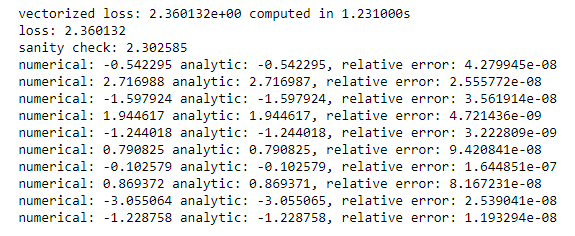
\includegraphics{images/cell3_output.PNG}}
\captionof{figure}{Output of cell 3}

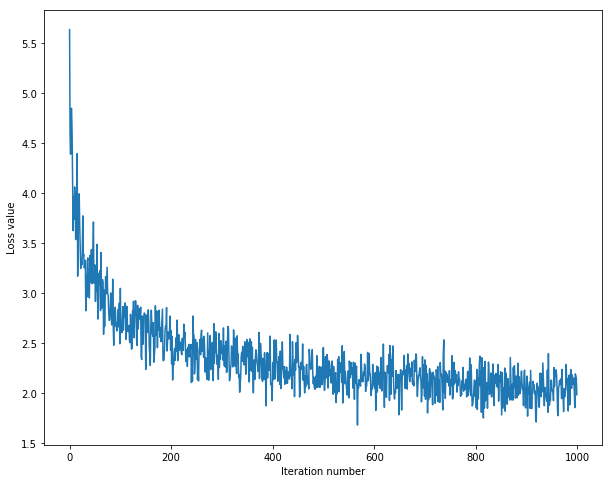
\includegraphics[width=0.75\textwidth]{images/training_loss.png}
\captionof{figure}{Training loss}
\end{minipage}
\newpage
\begin{minipage}[t]{\linewidth}
	\centering
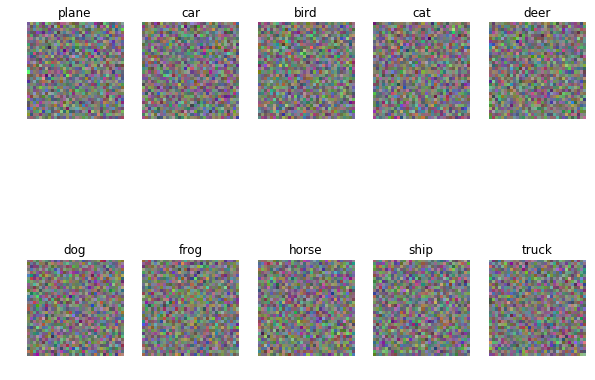
\includegraphics[width=0.75\textwidth]{images/visualization.png}
\captionof{figure}{Weight visualizations}
\end{minipage}
The weight visualizations do not correspond well with their respective classes. This indicates that the network hasn't learnt the representations of the classes.
\newpage

	\item We will prove this using the definition of convexity, i.e. $L(W)$ is convex if and only if $L(\lambda W_1 + (1 - \lambda)W_2) \leq \lambda L(W_1) + (1 - \lambda) L(W_2), \forall \lambda \in [0,1]$. \\\\
	Let $w_{1i}$ and $w_{2i}$ denote the $\text{i}^{th}$ rows of $W_1$ and $W_2$ respectively.
	\begin{align}
	L(\lambda W_1 + (1 - \lambda)W_2) &= -\log \frac{e^{(\lambda w_{1y} + (1 - \lambda)w_{2y})x}}{\sum_k e^{(\lambda w_{1k} + (1 - \lambda)w_{2k})x}}
	\end{align}
	\begin{align}
	\lambda L(W_1) + (1 - \lambda) L(W_2) &= -\lambda\log\frac{e^{w_{1y}x}}{\sum_k e^{w_{1k}x}} - (1 - \lambda)\log\frac{e^{w_{2y}x}}{\sum_k e^{w_{2k}x}} \\
	&= -\log\frac{e^{\lambda w_{1y}x}}{(\sum_k e^{w_{1k}x})^{\lambda}} - \log\frac{e^{(1 - \lambda)w_{2y}x}}{(\sum_k e^{w_{2k}x})^{(1 - \lambda)}} \\
	&= -\log \frac{e^{(\lambda w_{1y} + (1 - \lambda)w_{2y})x}}{(\sum_k e^{w_{1k}x})^{\lambda}(\sum_k e^{w_{2k}x})^{(1 - \lambda)}}
	\end{align}
	As the numerator in (1) and (4) is the same, we just have to prove that $\log \sum_k e^{(\lambda w_{1k} + (1 - \lambda)w_{2k})x} \leq \log (\sum_k e^{w_{1k}x})^{\lambda}(\sum_k e^{w_{2k}x})^{(1 - \lambda)}$. Since $\log x$ is monotone increasing, it is enough to prove that $\sum_k e^{(\lambda w_{1k} + (1 - \lambda)w_{2k})x} \leq (\sum_k e^{w_{1k}x})^{\lambda}(\sum_k e^{w_{2k}x})^{(1 - \lambda)}$. Let $e^{w_{1k}x} = u_k$ and $e^{w_{2k}x} = v_k$. From Holder's inequality,
	\begin{align}
	\sum_{i=1}^n x_i y_i &\leq \left(\sum_{i=1}^n|x_i|^p\right)^{\frac{1}{p}} . \left(\sum_{i=1}^n|y_i|^q\right)^{\frac{1}{q}} \\
	\text{where } \frac{1}{p} + \frac{1}{q} &= 1
	\end{align}
	Applying this inequality to $\sum_k e^{(\lambda w_{1k} + (1 - \lambda)w_{2k})x}$,
	\begin{align}
	\sum_k u_k^\lambda v_k^{(1 - \lambda)} &\leq \left(\sum_k u_k^{\lambda . \frac{1}{\lambda}}\right)^\lambda \left(\sum_k v_k^{(1 - \lambda) . \frac{1}{(1 - \lambda)}}\right)^{(1 - \lambda)} \\
	\implies \sum_k e^{(\lambda w_{1k} + (1 - \lambda)w_{2k})x} &\leq (\sum_k e^{w_{1k}x})^{\lambda}(\sum_k e^{w_{2k}x})^{(1 - \lambda)}
	\end{align}
	Hence, $L(.)$ is convex in $W$.
	
\end{enumerate}

\end{document}
